 \documentclass{include/protokollclass}
% Main File - Based on protokollclass.cls
% Comments are mostly in English (and some in German, concerning the Praktikum)
% ------------------------------------------------------------------------------
% Further files in folder:
%  - include/cmds.tex (for macros and additional commands)
%  - include/kitlogo.pdf (for titlepage)
%  - lit.bib (bibtex bibliography database)
%  - include/titlepage.tex (for layout of titelpage)
% ------------------------------------------------------------------------------
% Useful Supplied Packages:
% amsmath, amssymb, mathtools, bbm, upgreek, nicefrac,
% siunitx, varioref, booktabs, graphicx, tikz, multicol

\usepackage{rotating}
\usepackage{icomma}
\usepackage{subfig}
\usepackage{pdfpages}
\usepackage[onehalfspacing]{setspace}


%% ---------------------------------------------
%% |    Informationen über dieses Protokoll    |
%% ---------------------------------------------
\newcommand{\praktikum}{P3}                % P1 oder P2
\newcommand{\semester}{WS17/18}            % z.B. "WS14/15" oder "SS15"

\newcommand{\wochentag}{Mi}                % Mo, Di, Mi oder Do
\newcommand{\gruppennr}{144}                % Zweistellige Gruppennummer

\newcommand{\nachnamea}{Friedrich}             % Nachname des ersten Praktikanten
\newcommand{\vornamea}{Tabea}               % Vorname des ersten Praktikanten
\newcommand{\nachnameb}{Stockmeier}              % Nachname des zweiten Praktikanten
\newcommand{\vornameb}{Lea}              % Vorname des zweiten Praktikanten

\newcommand{\emailadressen}{lea.stockmeier@web.de, tabea.friedrich@t-online.de}
% optionale Angabe von Emailadresse(n) für den Kontakt mit dem Betreuer

\newcommand{\versuch}{Gravimetrie} % Name des Versuchs
\newcommand{\versuchsnr}{00}               % bitte die korrekte Nummer dem 
                                           % Arbeitsplatz am Versuchstag 
                                           % entnehmen
\newcommand{\fehlerrechnung}{Ja}         % Ob Fehlerrechnung im Versuch 
                                           % durchgeführt wurde oder nicht

\newcommand{\betreuer}{Betreuer}      % Name des zuständigen Betreuers
\newcommand{\durchgefuehrt}{00.00.17}      % Datum, an dem der Versuch 
                                           % durchgeführt wurde





%% --------------------------------------
%% |    Settings for Word Separation    |
%% --------------------------------------
% Help for separation:
% In German package the following hints are additionally available:
% "- = Additional separation
% "| = Suppress ligation and possible separation (e.g. Schaf"|fell)
% "~ = Hyphenation without separation (e.g. bergauf und "~ab)
% "= = Hyphenation with separation before and after
% "" = Separation without a hyphenation (e.g. und/""oder)

% Describe separation hints here:
\hyphenation
{
    über-nom-me-nen an-ge-ge-be-nen
    %Pro-to-koll-in-stan-zen
    %Ma-na-ge-ment  Netz-werk-ele-men-ten
    %Netz-werk Netz-werk-re-ser-vie-rung
    %Netz-werk-adap-ter Fein-ju-stier-ung
    %Da-ten-strom-spe-zi-fi-ka-tion Pa-ket-rumpf
    %Kon-troll-in-stanz
}





% um die Titelseite per PDF-reader auszufüllen. Vorgefertigte Daten
% können in Datei 'data.tex' modifiziert werden.
%\setboolean{forminput}{true}
% um die Anmerkungen zu den Textfeldern anzeigen zu lassen
%\setboolean{showannotations}{true}
% Erneuern der Seitenzahl in jedem Kapitel
%\setboolean{chapResetPageNumb}{true}
% Einbinden der Kapitelnummer in der Seitenzahl
%\setboolean{chapWiseNumb}{true}
% english or ngerman (new german für neue deutsche Rechtschreibung statt german)
\SelectLanguage{ngerman}

\title{Geophysikalische Geländeübungen \\ SS 2018 \\ Gravimetrie}
\subtitle{Messgebiet A59/1 (Riedheim)}
\author{\\ Svenja Müller \\ mueller-svenja@gmx.net
\\ \\und\\ \\
Lea Stockmeier \\ lea.stockmeier@web.de \\ \\ \\
Betreuer: Vorname1 Nachname1 und Vorname2 Nachname2}
\date{\vfill\vfill\vfill \today}


%% -----------------------
%% |    Main Document    |
%% -----------------------
\begin{document}
    % Titlepage und ToC
    \FrontMatter
    \maketitle


    \begingroup \let\clearpage\relax    % in order to avoid listoffigures and
    \tableofcontents                    % listoftables on new pages
    \listoffigures
%   \listoftables
    \endgroup
    %\cleardoublepage



    % Contents
    \MainMatter
    
    %\emptychapter[1]{Messprotokoll 1}{} % usage: \emptychapter[page displayed 
                                        %        in toc]{name of the chapter}
    %\pseudochapter[3]{Messprotokoll 2}  % usage: \pseudochapter[number of pages 
                                        %        added]{name of the chapter}
    
 %   \pseudochapter[2]{Versuchsbeschreibung}
%    \pseudochapter[4]{Messprotokoll}
    \chapter{Theoretische Grundlagen}
    \section{kjgkjgr}
    \chapter{Versuchsbeschreibung}
    %Versuchsbeschreibung
In der Geoelektrik wurden drei verschiedene Messmethoden verwendet. Das sind die Wenner-Kartierung, Schlumberger-Sondierung und die Tomographie. Sowohl die Wenner-Kartierung als auch die Tomographie wurde über dem Basaltgang durchgeführt, um diese Messmethode mit den übrigen vergleichen zu können.

In Abbildung \ref{abb:PBasalt} sind die Profile der Wenner-Kartierung und Tomographie abgebildet. Die Wenner-Kartierung wurde entlang E11-E12 durchgeführt und das Profil der Tomographie ist in dieser Abbildung beschriftet. Zu sehen ist, dass das Profil der Geoelektrik über dem Profil der Magnetik und Gravimetrie liegt. Dadurch kann man direkt die Messergebnisse vergleichen und eventuell sehen, welche Methode sich zum Untersuchen des Basalts eignet und welche nicht.

Die Schlumberger-Sondierung wurde auf dem gleichen Profil wie die Seismik-Messung mit Sissy durchgeführt, um die beiden Messungen vergleichen zu können. Dieses Profil ist das obere Profil E21-E22 in Abbildung \ref{abb:PWiese}.

%%%%%%%%%%%%%%%%%%%%%%%%%%%%%%%%%%%%%
\begin{figure}[ht]
\centering
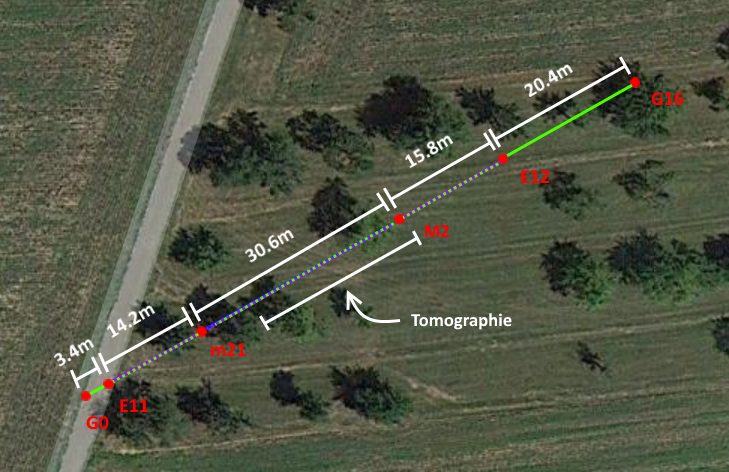
\includegraphics[width=0.6\textwidth]{fig/ElektrikMagnetikGravimetrie0gps.png}
\caption[Profile der Geoelektrik, Gravimetrie und Magnetik des Messgebiets am Basaltgang]{Profile der Geoelektrik, Gravimetrie und Magnetik des Messgebiets am Basaltgang. Die Graphik wurde von Rebekka Kirchgässner und Luisa Rank übernommen.}
\label{abb:PBasalt}
\end{figure}
%%%%%%%%%%%%%%%%%%%%%%%%%%%%%%%%%%%%

%%%%%%%%%%%%%%%%%%%%%%%%%%%%%%%%%%%%%
\begin{figure}[ht]
\centering
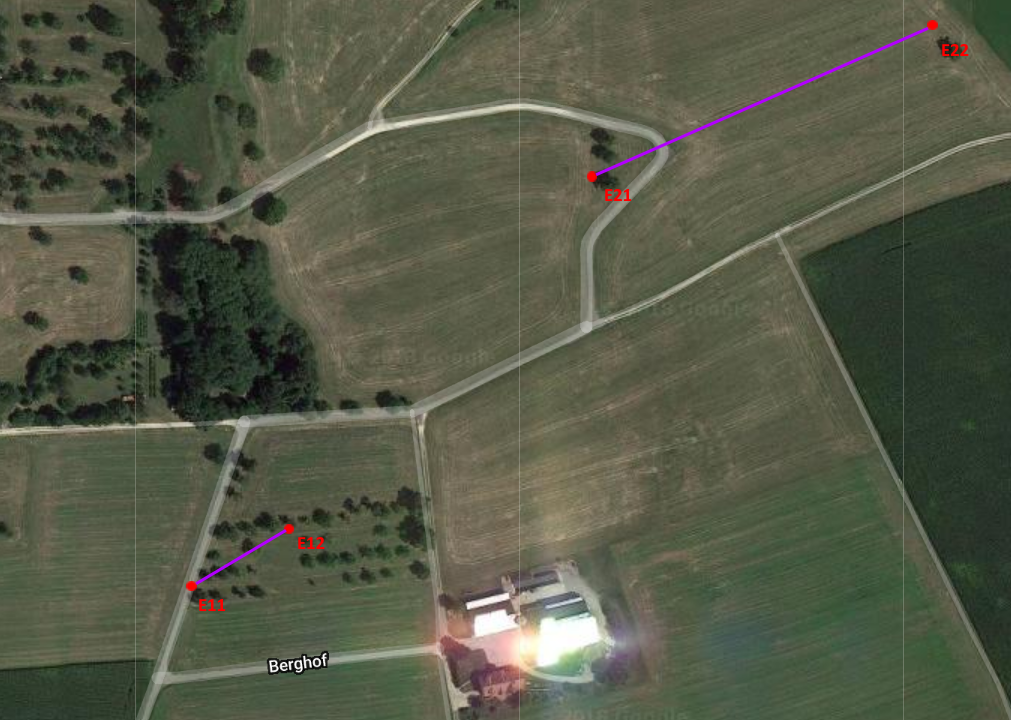
\includegraphics[width=0.6\textwidth]{fig/profilegps.PNG}
\caption[Profil E11-E12 und E21-E22 auf den beiden Messgebieten]{Profil E11-E12 und E21-E22 auf den beiden Messgebieten. Die Graphik wurde von Rebekka Kirchgässner und Luisa Rank übernommen.}
\label{abb:PWiese}
\end{figure}
%%%%%%%%%%%%%%%%%%%%%%%%%%%%%%%%%%%%
\newpage

\section{Wenner-Katierung}

Begonnen wurde mit der Wenner-Kartierung, um die Lage des Basaltgangs genauer zu bestimmen. Damit wir die Tomographie möglichst genau über dem Gang durchführen
können. 
Des weiteren soll eingeschätzt werden, wie gut diese Methode zum Vermessen des Basaltgangs geeignet ist.

Die Kartierung wurde in einer Tiefe von 5\,m vorgenommen. Dies ist begründet mit der Annahme, dass der Basaltgang vermutlich in ca. 1-2\,m Tiefe beginnt und nach unten 
als unendlich angenommen werden kann. Je mehr Basalt im Bereich der Messung ist, desto größer ist die Auswirkung auf die Ergebnisse.
Die Anordnung ist orthogonal zum Basaltgang und wird auch orthogonal dazu verschoben. Orientiert wurde sich dabei an der Messung von Magnetik, es wurde 
entlang des Magnetik-Profils M2-M21 gemessen. Dabei wurde darauf geachtet, dass auch eine Messung komplett außerhalb 
des Einflussbereichs des Basalt liegt.

\section{Tomographie}

Die Tomographie ist eine Kombination der ersten beiden Messmethoden. Sie wurde auf dem gleichen Profil wie die Wenner-Kartierung durchgeführt.
Es wurden 48 Elektroden verwendet, die in einem Abstand von 50\,cm, auf der gleichen Messlinie wie bei der Wenner-Kartierung aufgestellt waren. 
Die Mitte der Messlinie wurde auf einen Punkt gesetzt, an dem auch die Mitte des Basaltgangs vermutet wurde. Insgesamt wurde also auf einer Länge von 24\,m gemessen.
Als 0-Punkt für die Messung wurde das obere Ende des Messbands festgelegt.
Nachdem die Elektroden aufgestellt und angeschlossen wurden, wurde die Messung automatisch mit einem Messgerät ausgeführt. Auf das Ergebnis musste ungefähr 
eine Stunde gewartet werden. Das Messprotokoll zur Tomographie befindet sich im Anhang unter der Abbildung \ref{abb:AnhTomographie}.

\section{Schlumberger-Sondierung}

Sie Schlumberger-Sondierung wurde nicht auf dem Messgebiet über dem Basaltgang vorgenommen, sondern auf einer Wiese wesentlich weiter oben. Auf dieser Wiese wurde 
bereits mit der Seismik gemessen. Um unsere Ergebnisse von der Seismik-Messung und dieser Messung vergleichen zu können, wurde die Messung entlang der gleichen
Linie durchgeführt.

Da wir kein sehr großes, gerades Gelände hatten und auch mit der Seismik in keinen großen Tiefen gemessen wurde, betrug die Länge des Profils 200\,m. Als Mitte 
haben wir den Punkt des Mittelschusses der Hammerschlag-Methode (Seismik) verwendet.
In der Mitte des Profils haben wir angefangen, die Elektroden zu stecken. In beide Richtungen haben wir den Abstand exponentiell vergrößert. Die genauen Abstände kann man dem Messprotokoll dieser Messung im Anhang entnehmen.

    % appendix for more or less interesting calculations
 %   \Appendix
 %   \chapter*{\appendixname} \addcontentsline{toc}{chapter}{\appendixname}
    % to make the appendix appear in ToC without number. \appendixname = 
    % Appendix or Anhang (depending on chosen language)
 %   \section{Messprotokolle}

\begin{figure}[h!]
 \centering
 \includegraphics[width=0.8\textwidth]{fig/Messprotokolle/Kalibrierung.png}
 \caption{Messprotokoll zur Kalibrierungsmessung}
 \label{fig:MPKalibrierung}
\end{figure}

\begin{figure}[h!]
 \centering
 \includegraphics[width=\textwidth]{fig/Messprotokolle/EinflussHuette.png}
 \caption{Messprotokoll zum Profil zur Untersuchung der Einflüsse äußerer Störfaktoren auf die Basismessung}
 \label{fig:MPHuette}
\end{figure}

% \begin{figure}[h!]
%  \centering
%  \includegraphics[width=\textwidth]{fig/Messprotokolle/}
%  \caption{}
%  \label{fig:}
% \end{figure} %\cleardoublepage



    % Bibliography
    \TheBibliography

    % BIBTEX
    % use if you want citations to appear even if they are not referenced to: 
    % \nocite{*} or maybe \nocite{Kon64,And59} for specific entries
    %\nocite{*}
    \bibliographystyle{babalpha}
    \bibliography{lit.bib}

    % THEBIBLIOGRAPHY
    %\begin{thebibliography}{000}
    %    \bibitem{ident}Entry into Bibliography.
    %\end{thebibliography}
\end{document}
